\documentclass[aspectratio=169,10pt]{beamer}
\usepackage{fontspec}
\usepackage{assets/ako-beamer}
\hypersetup{colorlinks=true,urlcolor=AKORed}

\title{AI, Human Cognition and Knowledge Collapse}
\author{John Barraza}
\institute{Universidad del Pacífico · AI Economic Modelling}
\date{September 2026}

\begin{document}

% 1
\begin{frame}[plain]
  \vspace{.55cm}
  {\color{AKORed}\large\bfseries REPOSITORY 04}\par\vspace{.35cm}
  {\usebeamerfont{title}\color{AKONavy}AI, Human Cognition and\\Knowledge Collapse}\par\vspace{.35cm}
  {\large Acemoglu, Kong \& Ozdaglar (2026)}\par\vspace{.6cm}
  \begin{tikzpicture}
    \draw[AKONavy,line width=2pt] (0,0)--(11.5,0);
    \draw[AKORed,line width=5pt] (8.2,0)--(11.5,0);
  \end{tikzpicture}
  \vfill
  {\small John Barraza · Universidad del Pacífico}\hfill{\small\href{https://github.com/johnbarraza/ai-04-acemoglu}{github.com/johnbarraza/ai-04-acemoglu}}
\end{frame}

% 2
\begin{frame}{1. The paper and the agent's problem}
\small
\begin{columns}[T,onlytextwidth]
  \column{.42\textwidth}
  \tagpill{Question}\par\vspace{.25cm}
  When can accurate, personalized AI improve decisions today yet erode the shared knowledge needed tomorrow?
  \vspace{.4cm}
  \begin{block}{One mechanism}
  Human effort jointly produces a private signal and a public externality. AI adds private precision only.
  \end{block}
  \column{.54\textwidth}
  \tagpill{Choice: $e\ge0$}\par\vspace{.15cm}
  \[
  \max_{e\ge0}\ \underbrace{f_{00}+G(X)\Delta_G+G(X)G(Y)\Delta_X}_{\text{expected task output}}
  -\frac{\varepsilon}{\varepsilon+1}e^{(\varepsilon+1)/\varepsilon},
  \]
  \[
  Y=\sigma^{-2}+\lambda_Ie+\tau_A,\quad
  \Delta_I=0,\ \Delta_X>0.
  \]
  For $X>0$, the unique interior optimum satisfies
  \[
  \Delta_XG(X)\lambda_Ig(Y)=e^{1/\varepsilon}.
  \]
\end{columns}
\paperref{May 5, 2026 PDF, Sections 3.1--3.5, equations (4)--(6).}
\end{frame}

% 3
\begin{frame}{2. Main result: one complement, one substitute}
\small
\textbf{Observation 1 (corrected domain).} Suppose Gaussian posterior errors, $X>0$, $Y>0$, $\lambda_I>0$, $\tau_A\ge0$, and Assumption 1 ($\Delta_I=0$, $\Delta_X>0$). With $G(z)=2\Phi(\sqrt z)-1$ and $g=G'$, then
\[
\boxed{U_{eX}=\Delta_X\lambda_Ig(X)g(Y)>0}
\qquad
\boxed{U_{e\tau_A}=\Delta_XG(X)\lambda_Ig'(Y)<0}.
\]
\begin{columns}[T,onlytextwidth]
  \column{.48\textwidth}
  \begin{block}{General knowledge $X$}
  Raises the payoff from learning the context: effort and public precision are complements.
  \end{block}
  \column{.48\textwidth}
  \begin{alertblock}{Agentic precision $\tau_A$}
  Enters the same precision index as private learning: AI and effort are substitutes.
  \end{alertblock}
\end{columns}
\vspace{.15cm}
\textbf{Implication.} The unique best response $e(X,\tau_A)$ rises in $X$ and falls in $\tau_A$, strictly for $X>0$.
\paperref{Observation 1 and Observation 2, pp. 13--15. The paper omits $X>0$ from the displayed cross-partial domain.}
\end{frame}

% 4
\begin{frame}{3. What I did: attack the zero-collapse hinge}
\small
\begin{columns}[T,onlytextwidth]
  \column{.54\textwidth}
  I restored the production term the paper never relaxes:
  \[
  \Delta_I>0\quad\Longrightarrow\quad
  U_e=\lambda_Ig(Y)\{\Delta_I+G(X)\Delta_X\}-e^{1/\varepsilon}.
  \]
  At the alleged collapse boundary,
  \[
  U_e(0;0,\tau_A)=\lambda_Ig(\sigma^{-2}+\tau_A)\Delta_I>0.
  \]
  Hence $e(0,\tau_A)>0$ and
  \[
  F(0)=\left[\Sigma^2+(\lambda_GIe(0,\tau_A))^{-1}\right]^{-1}>0.
  \]
  \column{.42\textwidth}
  \begin{alertblock}{Economic consequence}
  Exact zero knowledge is no longer a fixed point. A low-knowledge trap may survive, but literal collapse does not.
  \end{alertblock}
  \begin{block}{Formal check}
  EconCSLib target: \texttt{AKO26KnowledgeCollapse}. Lean checks the algebraic/order core; source fidelity remains a separate audit.
  \end{block}
\end{columns}
\paperref{Original extension; baseline Assumption 1 and Sections 5.1--5.3.}
\end{frame}

% 5
\begin{frame}{4. Where I did not believe the AI}
\begin{columns}[T,onlytextwidth]
  \column{.48\textwidth}
  \IfFileExists{hand/derivation.jpg}{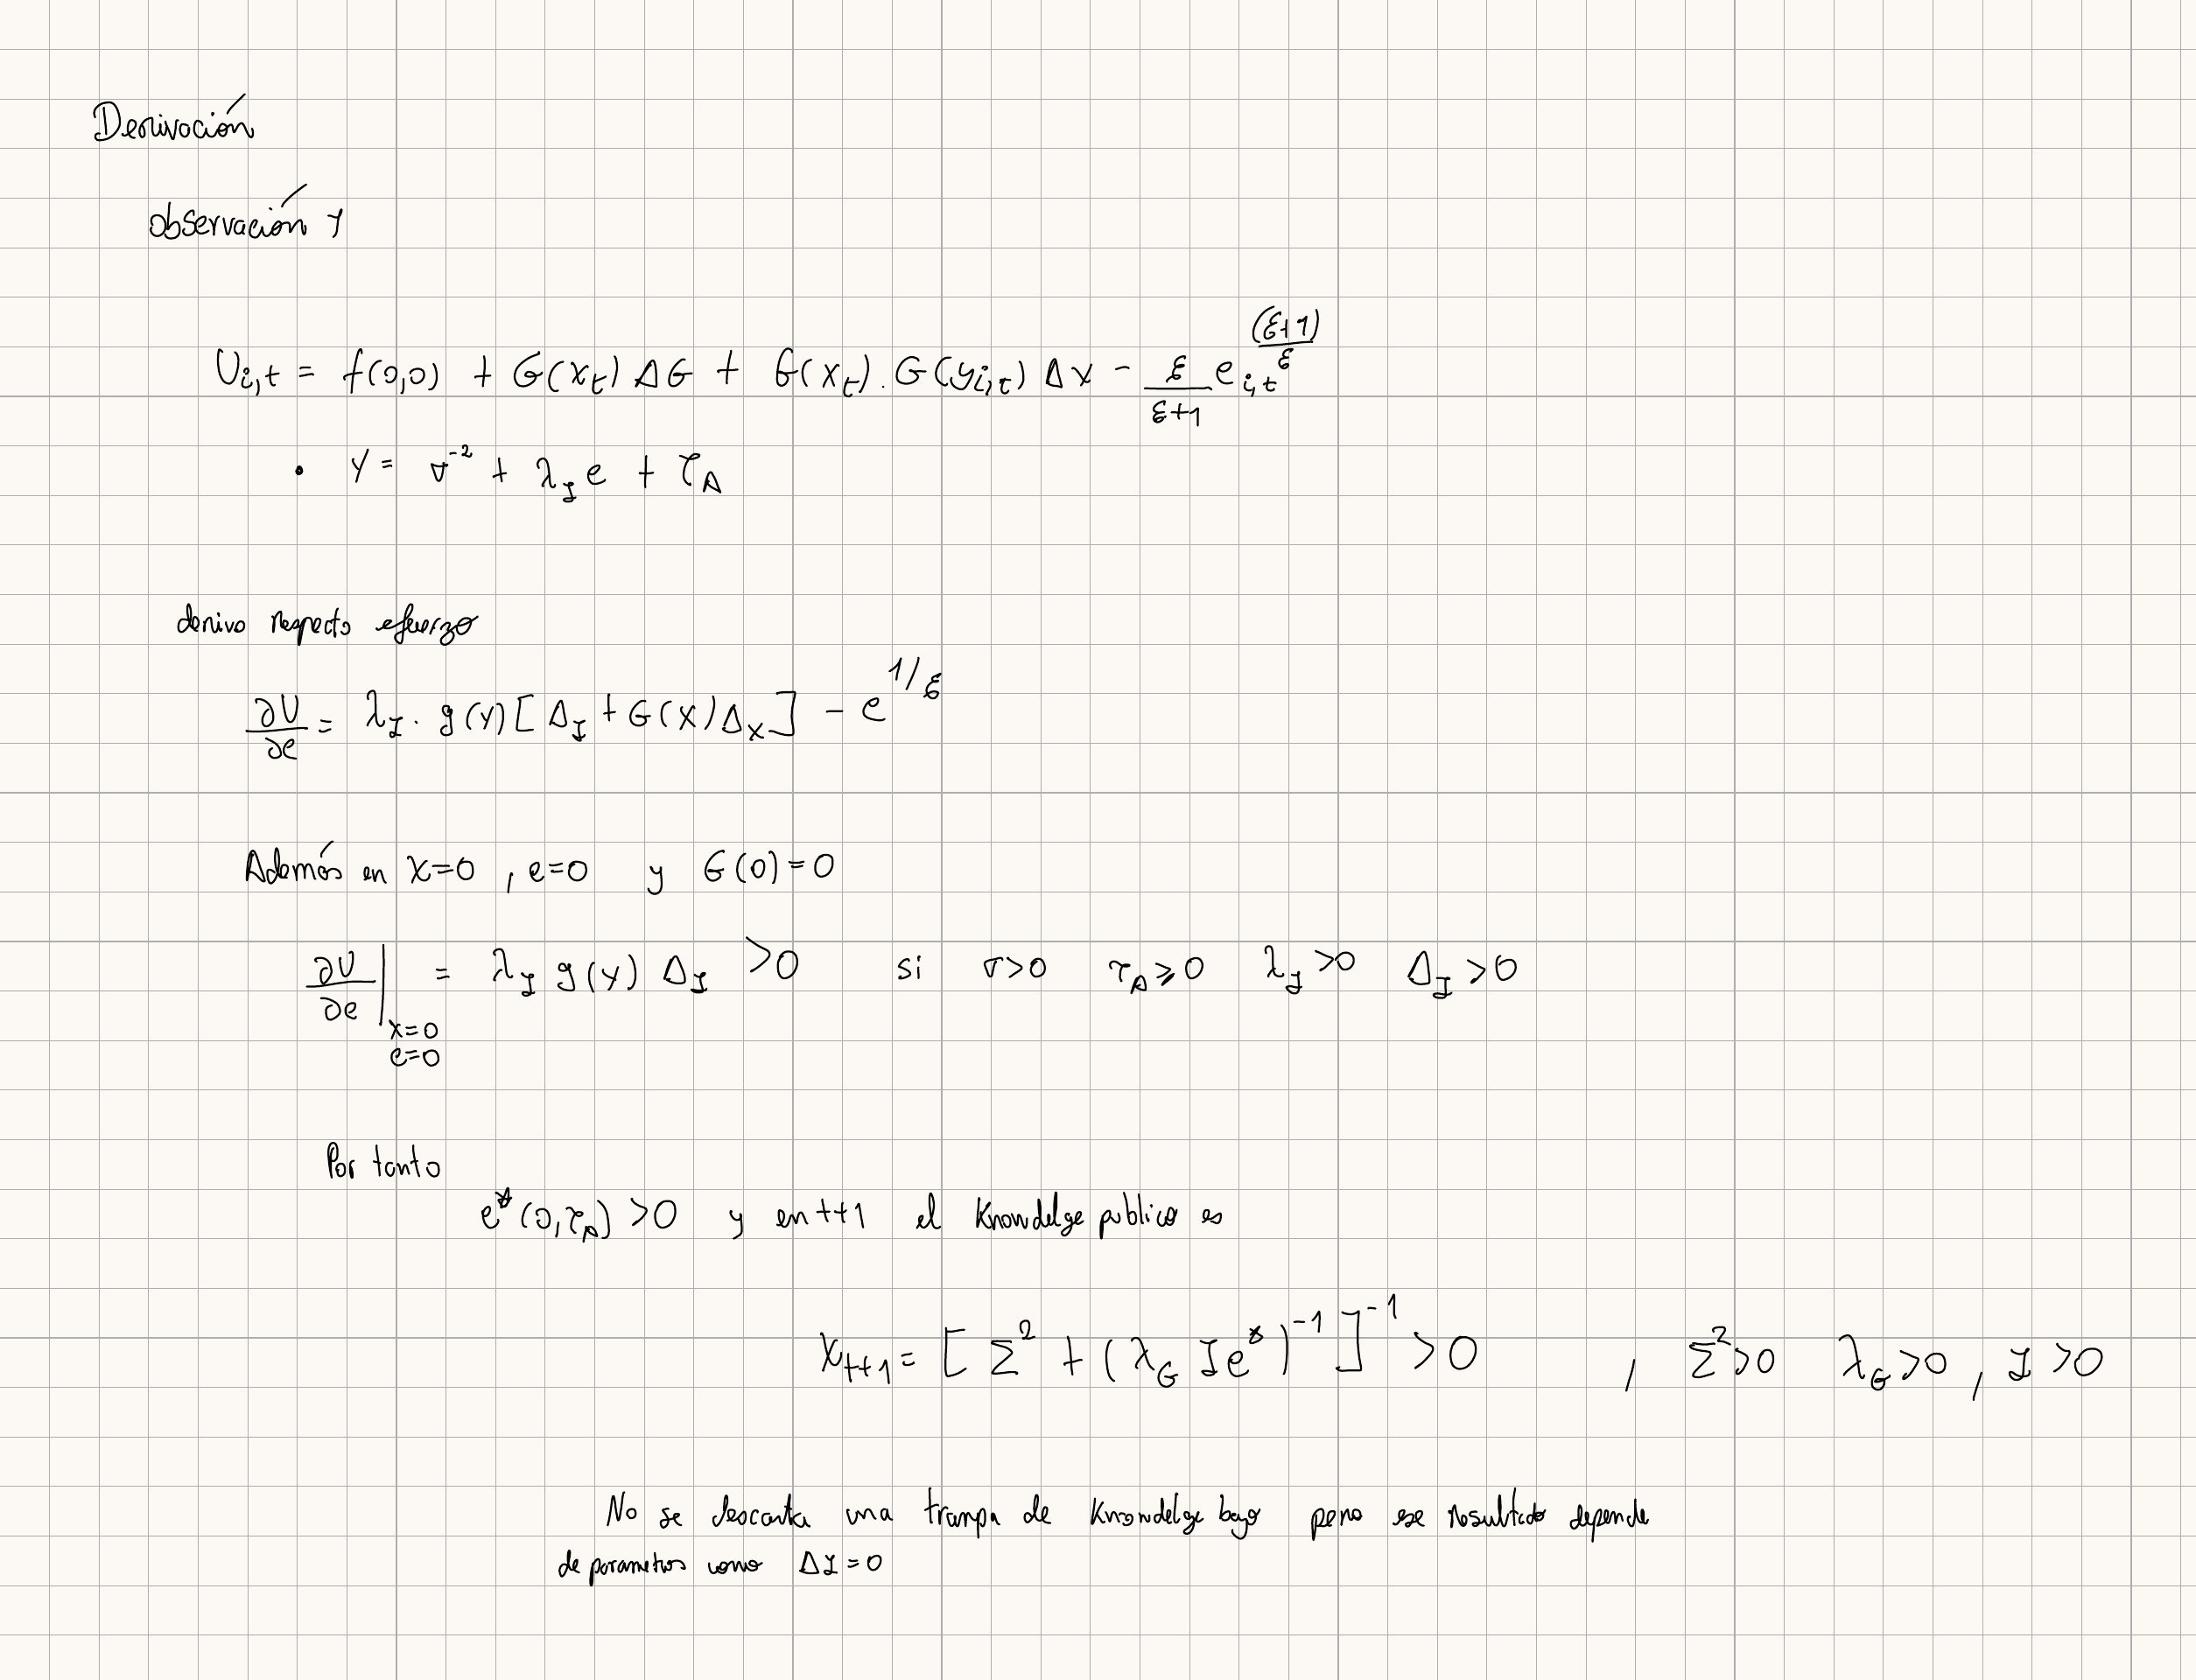
\includegraphics[width=\linewidth,height=5.5cm,keepaspectratio]{hand/derivation.jpg}}{%
    \begin{tikzpicture}\node[draw=AKORed,fill=AKORedPale,text width=.88\linewidth,minimum height=5.2cm,align=center] {\Large Add your own\\hand derivation\\\vspace{.3cm}\normalsize\texttt{hand/derivation.jpg}};\end{tikzpicture}}
  \column{.48\textwidth}
  \verdictbox{The sign calculation is correct on $X>0$, but it does not identify something unique to an \emph{agent}: any context-specific precision shock added to $Y$ crowds out effort.}
  \vspace{.3cm}
  The stronger claim—complete destruction of useful knowledge—leans on $\Delta_I=0$. It is better read as a sharp benchmark for a low-knowledge trap.
  \vspace{.3cm}
  \textbf{Two slips to remember:}
  \begin{itemize}
    \item $g(X)$ is not finite at the endpoint $X=0$;
    \item Proposition 5 leaves $\tau_A=\tau_A^c$ unstated.
  \end{itemize}
\end{columns}
\paperref{Own derivation and audit against the May 5, 2026 PDF.}
\end{frame}

\end{document}
